\chapter{Analyse}
Die Analyse konzentriert sich auf das Software Engineering. In den folgenden Abschnitten werden Analyse, Aufbau sowie die Umsetzung und Schlussfolgerungen erläutert.
\\

Als Grundlage für die RadioTour Applikation dient aus Sicht der Funktionalität die bestehende Web Applikation. Daraus wurden die Requirements und UseCases erzeugt. Im folgenden werden die einzelnen Teile der Analyse vorgestellt.

\section{Struktur der Applikation}
%ja, plural ist Status, http://de.wikipedia.org/wiki/Status
Die Applikation hat im Grunde zwei Status, vor dem Rennen die Aufnahme durch einen Import der Informationen und beim Rennen bei der Aufzeichnung der Veränderungen. Diese können aber nicht absolut voneinander getrennt werden, da während dem Rennen Änderungen denkbar sind. So entsteht die Baumartige Struktur, wie sie in der Abbildung zu sehen ist.

\begin{figure}[h!]
\caption{Struktur der Applikation}
\centering
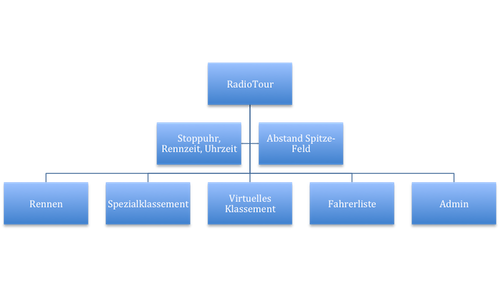
\includegraphics{technischerbericht/analyse/images/struktur.png}
\end{figure} 


\section{Technologien}
Die native Programmiersprache für das Android Betriebssystem ist Java. Um die Hardware optimal zu nutzen haben wir uns für eine native Entwicklung entschieden. Dies bringt den Vorteil, dass auf die gesamte \gls{api} zugegriffen werden kann.

\subsection{Entwicklungsumgebung}
Die von Android vorgeschlagene Entwicklungsumgebung ist Eclipse mit einem Plugin für Entwicklung von Android Applikationen. Auf der Entwicklerseite von Android steht dazu folgendes:
\begin{quote}
Android Development Tools (ADT) is a plugin for the Eclipse IDE that is designed to give you a powerful, integrated environment in which to build Android applications.
\footnote{\url{http://developer.android.com/sdk/eclipse-adt.html}}
\end{quote}
Eclipse ist eine weit verbreitete \gls{ide} und wird aktiv weiter entwickelt. Mit dem Plugin zusammen bilden Sie eine solide Grundlage für unser Projekt.
\\
Damit die Android Applikation direkt auf dem Computer getestet werden kann, stellt Google ein Simulator für Tablets zur Verfügung. Der Simulator ist allerdings auch als solcher zu betrachten. Die Bedienung ist nicht vergleichbar mit einem richtigen Tablet und ersetzt es auch nicht. Daher haben wir für die Entwicklung zusätzlich auch das ThinkPad Tablet verwendet.

\subsection{Android Version}
Eine Anwendung wird für eine spezifische Android Version entwickelt und getestet, somit kann garantiert werden, dass das Verhalten der Anwendung  immer gleich ist. In dieser Arbeit ist dies die Version 3.1 mit dem Versionsnamen \textit{Honeycomb}.

\section{Architektur}
Lorem ipsum dolor sit amet, consetetur sadipscing elitr, sed diam nonumy eirmod tempor invidunt ut labore et dolore magna aliquyam erat, sed diam voluptua. At vero eos et accusam et justo duo dolores et ea rebum. Stet clita kasd gubergren, no sea takimata sanctus est Lorem ipsum dolor sit amet. Lorem ipsum dolor sit amet, consetetur sadipscing elitr, sed diam nonumy eirmod tempor invidunt ut labore et dolore magna aliquyam erat, sed diam voluptua. At vero eos et accusam et justo duo dolores et ea rebum. Stet clita kasd gubergren, no sea takimata sanctus est Lorem ipsum dolor sit amet.

\section{Realisierung}
Lorem ipsum dolor sit amet, consetetur sadipscing elitr, sed diam nonumy eirmod tempor invidunt ut labore et dolore magna aliquyam erat, sed diam voluptua. At vero eos et accusam et justo duo dolores et ea rebum. Stet clita kasd gubergren, no sea takimata sanctus est Lorem ipsum dolor sit amet. Lorem ipsum dolor sit amet, consetetur sadipscing elitr, sed diam nonumy eirmod tempor invidunt ut labore et dolore magna aliquyam erat, sed diam voluptua. At vero eos et accusam et justo duo dolores et ea rebum. Stet clita kasd gubergren, no sea takimata sanctus est Lorem ipsum dolor sit amet.

\section{Testing}
Lorem ipsum dolor sit amet, consetetur sadipscing elitr, sed diam nonumy eirmod tempor invidunt ut labore et dolore magna aliquyam erat, sed diam voluptua. At vero eos et accusam et justo duo dolores et ea rebum. Stet clita kasd gubergren, no sea takimata sanctus est Lorem ipsum dolor sit amet. Lorem ipsum dolor sit amet, consetetur sadipscing elitr, sed diam nonumy eirmod tempor invidunt ut labore et dolore magna aliquyam erat, sed diam voluptua. At vero eos et accusam et justo duo dolores et ea rebum. Stet clita kasd gubergren, no sea takimata sanctus est Lorem ipsum dolor sit amet.

\section{Ergebnisse und Schlussfolgerungen}
Lorem ipsum dolor sit amet, consetetur sadipscing elitr, sed diam nonumy eirmod tempor invidunt ut labore et dolore magna aliquyam erat, sed diam voluptua. At vero eos et accusam et justo duo dolores et ea rebum. Stet clita kasd gubergren, no sea takimata sanctus est Lorem ipsum dolor sit amet. Lorem ipsum dolor sit amet, consetetur sadipscing elitr, sed diam nonumy eirmod tempor invidunt ut labore et dolore magna aliquyam erat, sed diam voluptua. At vero eos et accusam et justo duo dolores et ea rebum. Stet clita kasd gubergren, no sea takimata sanctus est Lorem ipsum dolor sit amet.